%!TEX program = xelatex
% 完整编译方法 1 pdflatex -> bibtex -> pdflatex -> pdflatex
% 完整编译方法 2: xelatex -> bibtex -> xelatex -> xelatex
\documentclass[lang=cn,11pt]{elegantpaper}

\title{A Network Embedding Augmented Collaborative Filtering Model For Recommendation}

\author{袁梦祥}
\institute{安徽大学大数据与云服务工程实验室}
\date{}

% 实现图片并排
\usepackage{subfigure}

% 算法表格
%\usepackage{algorithm}  
%\usepackage{algpseudocode}  
%\usepackage{amsmath}  
%\renewcommand{\algorithmicrequire}{\textbf{Input:}}  
%\renewcommand{\algorithmicensure}{\textbf{Output:}}

\begin{document}

\maketitle

\begin{abstract}
\noindent 使用推荐系统为用户提供个性化的推荐服务,有助于提高用户的满意度,更好的发掘物品的“长尾”,推荐系统的核心是推荐算法,基于协同过滤的推荐算法是目前应用比较广泛的推荐算法。但传统的协同过滤算法
在推荐时存在数据稀疏量大,数据维数高,无法利用内容信息等问题,为了解决协同过滤算法的缺点,本文引入
了网络表示学习的方法,使用二部图网络来表示用户的行为数据和项目的内容数据,再通过针对二部图结构设计
的网络表示学习方法,学习网络中节点的低维度潜在表示,在低维嵌入空间考虑用户和项目的领域信息,结合矩阵分解模型为用户进行基于评分的推荐。
本文结合协同过滤模型和网络表示学习的优点,同时考虑项目的内容特征和用户的行为偏好,
提出了一种新的考虑嵌入表示的加强矩阵分解推荐算法。我们在GoodBooks和Movielens数据集上对此方法进行
了实验验证,结果表明,我们的算法有更好的推荐效果。
\keywords{推荐系统,二部图网络,网络表示学习,矩阵分解,协同过滤 }
\end{abstract}


\section{引言}

在当今竞争激烈的市场环境下,产品的个性化程度已经成为影响顾客产品选择和满意度的重要因素。如果要给用户提供个性化的商品或服
务,就必须充分研究用户的兴趣,而这正是推荐系统主要解决的问题,通过挖掘用户的历史行为数据,推荐系统可以自动发现用户的个性
化需求。

推荐系统的本质是通过一定的方式将用户和项目联系起来,研究怎么将用户兴趣和项目关联起来的推荐算法是整个推荐系统的核心。
目前应用最广泛的推荐算法是协同过滤的推荐算法,学术界有许多关于该算法的研究\cite{Linden2003,Miranda2009,Sarwar2001a,Su2009}。
在实际应用中用户的行为数据通常非常稀疏,矩阵分解是最常用的基于模型的协同过滤算法\cite{Salakhutdinov2007,Koren2009},
该算法通过用户-项目二部图网络,同时学习用户和项目的潜在表示。传统的矩阵分解在嵌入表示顶点时,使用线性变换将网络顶点嵌入到低维空间。
最近的研究趋势是使用深度学习的方法学习网络上的顶点嵌入\cite{He2017}进行推荐。在为推荐而构建的用户-项目二部网络中,
虽然边只存在于不同类型的顶点之间,但同一类型的顶点之间存在隐式关系,例如在用户之间就存在一种隐式的关系,
这种关系表明用户对同一项目的偏好。最近有论文指出,对这种隐式关系进行建模可以提高推荐性能\cite{Yu2018}。
然而,现有的网络表示学习方法\cite{Perozzi2014,Grover2016,Tang2015}仅仅对二部图中的显式关系进行了建模而忽略潜在的隐式关系。
与现有的协同过滤模型用于推荐的工作不同,我们结合网络表示学习的方法,在嵌入表示顶点时充分考虑二部图网络结构的特点。
最后在生成推荐时,不仅考虑用户的行为信息,同时利用到项目的内容信息,可以比以前的方法产生更好的预测。

总之,本文的主要贡献有两方面:
\begin{itemize}
    \item 在嵌入表示顶点时充分考虑二部图网络结构的特点。
    通过项目用户/项目二部图数据学习用户顶点的嵌入表示,通过项目/标签二部图数据学习项目顶点的嵌入表示,
    在低维嵌入空间中考虑用户行为和项目内容的领域信息;
	
    \item 提出了一种改进的预测方法,该方法基于矩阵分解技术与网络表示学习技术,联合训练用户的行为和项目内容的领域信息,
    对原始评分矩阵进行填充,为用户产生基于预测评分的推荐。
\end{itemize}

本文的其余部分安排如下。第二节介绍了相关的工作; 第三节详细介绍了推荐算法的整体架构; 第四节介绍了实验; 最后,第五节总结论文并讨论论文的未来工作。

\section{相关工作}

我们的工作涉及到协同过滤和基于网络表示学习的推荐。因此,在本节中,我们将简要回顾这些领域的相关工作。

\subsection{协同过滤}

基于用户的历史行为数据对用户产生推荐的方法主要是基于协同过滤思想\cite{Su2009},矩阵分解是实现协同过滤最常用的方法,它可以很好的解决冷启动问题\cite{Qiu2011}。
但基本的矩阵分解模型,如\cite{Salakhutdinov2007,Koren2009},完全通过用户-项目的二部图数据,学习用户和项目的潜在表示,使用用户-项目潜在特性的点乘操作预测用户对项目的评分。
\cite{Koren2008}将邻域信息集成到矩阵分解中。它假定用户对某一项的评价不仅由用户对该项的潜在表示决定,而且还由用户对其他项的评价行为构成,即考虑物品
的邻域信息。这种方法在许多领域的性能都优于传统的矩阵分解模型,然而这种算法在建模时使用线性变换将网络顶点嵌入到低维空间,没法捕捉用户与项目的非线性关系,
而且仅仅考虑了用户的行为信息,没有考虑项目的内容信息。

\subsection{基于网络表示学习的推荐}

在推荐系统中,用户和项目形成一个二部网络,边包含丰富的协同过滤模式的用户评价行为\cite{He2017a}。基于网络表示的推荐算法利用网络的结构信息,
使用非线性变换将网络顶点嵌入到低维空间,学习网络中顶点的低维表示进行推荐\cite{Pongnumkul2018,Liu2009},可以捕捉用户与项目的非线性关系。
开创性的DeepWalk\cite{Perozzi2014}和Node2vec\cite{Grover2016}算法对同质网络进行建模,
有一些后续工作是利用同质顶点之间的高阶邻近来嵌入同构网络,例如 LINE \cite{Tang2015}学习了一阶和二阶关系的两个分离嵌入。
这类算法的基本思想是通过随机游走将网络转换为顶点序列的语料库。尽管这种方式具备有效性和普遍性,但\cite{Gao2018}指出这些方法
忽略了二部图网络的特殊性质,对于嵌入表示二部图网络可能不是最理想的。而且现有的网络表示学习的工作主要集中在嵌入表示同质网络,
网络中的顶点都是相同类型的\cite{Grover2016,Perozzi2014,Liao2018},仅仅是对二部网络中的显式关系进行建模,而且在产生推荐时没有考虑项目的内容信息。

\section{推荐模型}

在本节中,我们将介绍我们的推荐模型,这是一种基于二部图嵌入表示和协同过滤的推荐模型。我们的模型通过利用两个异构信息源,
分别是项目的标签信息和用户的评分信息,来预测用户对项目的评分。在下文中,我们首先详细介绍了我们的推荐框架,
然后是分别介绍数据的预处理过程,二部图的嵌入表示算法,以及在分别获得用户和项目的嵌入表示后,怎么进行联合训练,获得最终的预测评分矩阵。

\subsection{算法框架}
推荐系统是根据用户过去的历史行为,为用户提供个性化的推荐服务。因此,在我们的推荐系统中需要使用到用户的历史评分信息,其次为了
获得项目的内容信息,我们需要使用项目/标签数据。

图\ref{fig:framwork}描述了我们所提出方法的基本思想。首先,对收集来的用户-项目评分文件进行预处理,
获得用户-项目的二部图表示,然后使用二部图网络嵌入算法进行获得用户的嵌入表示。接下来,
同样处理项目-标签文件以获得项目的嵌入表示,最后使用改进后的矩阵分解模型,联合训练两个向量,
使用预测评分填充评分矩阵,对用户进行个性化推荐

\begin{figure}[t]
	\centering
	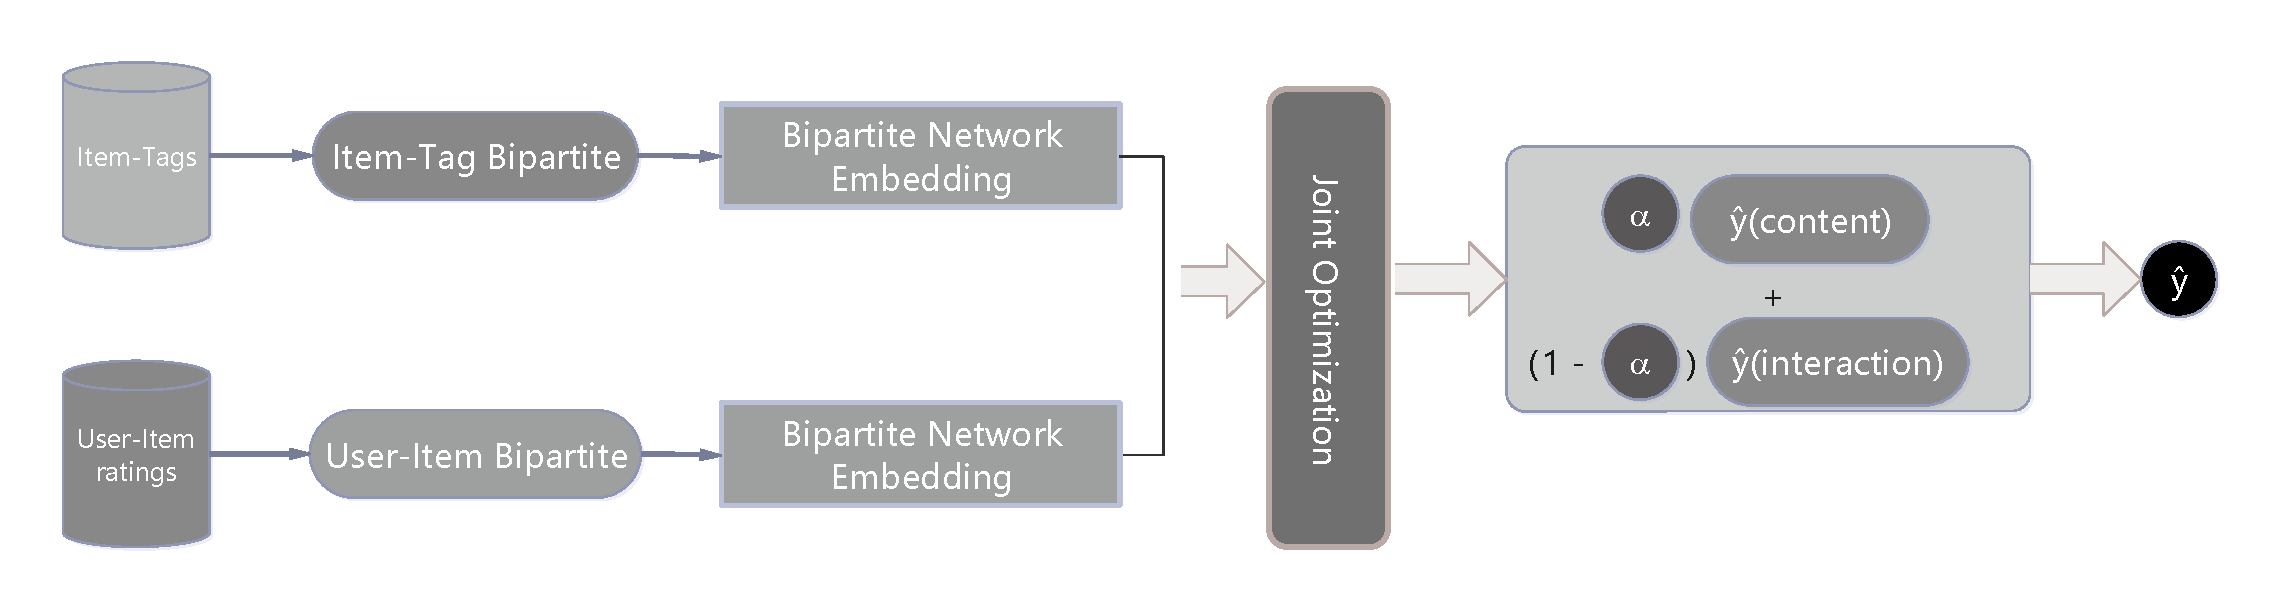
\includegraphics[width=1.0\textwidth]{imgs/framework.pdf}
	\caption{recommendation framework \label{fig:framwork}}
\end{figure}

\subsection{数据预处理}

从原始的文本数据到可以进行二部图嵌入表示的二部图数据需要经过数据的预处理过程,我们的的算法使用到了user-item的评分数据和item-tag内容数据。
针对用户的评分数据,我们很容易的可以使用二部图进行表示。如图\ref{fig:matrix},左边的图为用户的评分矩阵图,
右边的图即为对应的用户物品二部图网络,其中圆形节点分别代表用户和项目,节点之间的边代表用户对物品存在打分行为,
边的权重代表对应的用户项目评分。类似的,对于项目标签数据,我们可以把项目和tag当作网络中的节点。


\begin{figure}[htbp]
	\centering
	\subfigure{
		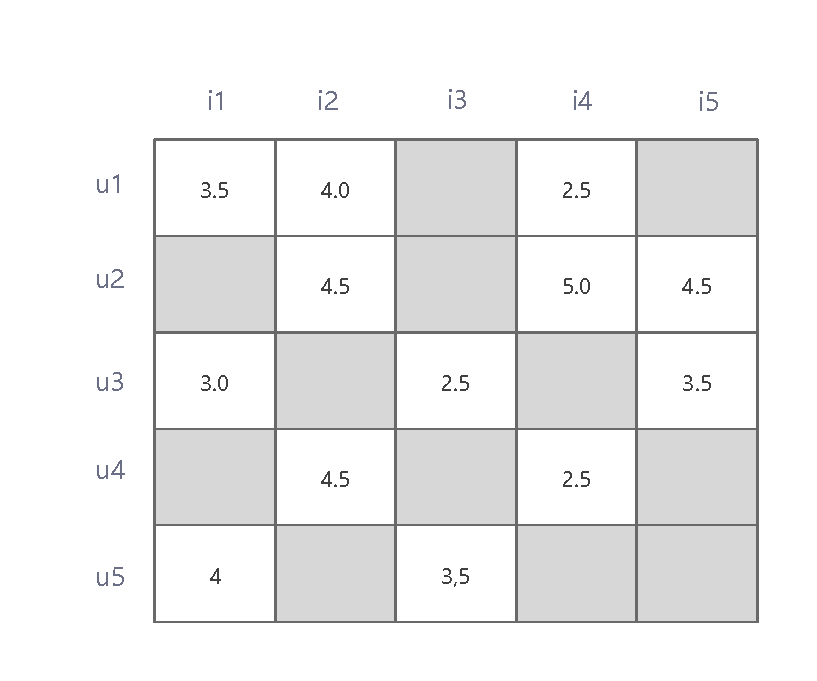
\includegraphics[width=0.4\textwidth]{imgs/matrix.pdf}
	}
	\quad
	\subfigure{
		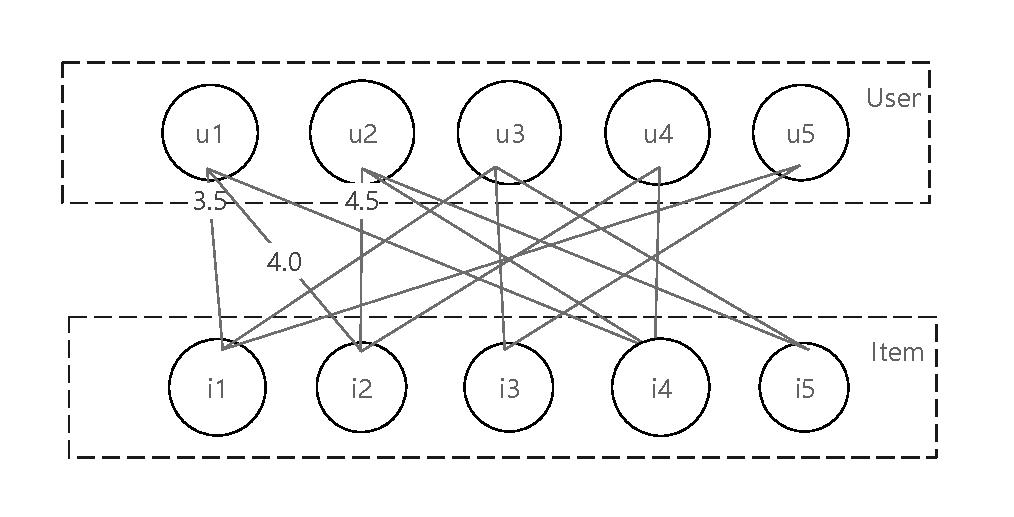
\includegraphics[width=0.4\textwidth]{imgs/matrix2.pdf}
    }

	\caption{ An example of the bipartite network structure\label{fig:matrix}} 
\end{figure}

\subsection{二部图嵌入表示}

Follow Ming Gao的工作\cite{Gao2018},我们使用BiNE的算法对二部图网络进行嵌入表示。
在本小节我们会对 BiNE 方法进行简要的概述。

良好的网络嵌入应该能够很好地重构原始网络。为了在二部网络实现这一目标,我们考虑从两个特征来重构二部网络,分别是由直接相连的边所代表的显式关系,和由未直接相连的传递链隐含的隐式关系,通过联合优化这两个目标函数来学习二部图顶点的嵌入:

\begin{equation} \label{equ:BiNE}
    maximize\ L=\alpha \log O_{2}+\beta \log O_{3}-\gamma O_{1}
\end{equation}

公式\ref{equ:BiNE}中$ O_{1}$ 代表对二部网络中的显示关系进行建模得到的最小化目标函数。
$ O_{2}$ 和 $ O_{3}$ 代表对二部网络中的隐式关系进行建模得到的最大化目标函数,
参数$ \alpha,\beta,\gamma$ 三个参数分别代表了联合训练时各部分的比例。
最后,为了优化联合模型,使用随机梯度上升算法(SGA)对模型进行训练,
获得最终的嵌入向量表示。

在本论文中,我们采取\cite{Gao2018}中的默认配置,分别对用户-项目二部图数据
和项目-标签二部图数据进行嵌入表示。

\subsection{联合训练}

矩阵分解是一种广泛采用的基于模型的协同过滤方法。它将用户项目评分矩阵分解为低秩矩阵以进行预测。这种因式分解的思想是同时获得用户和项目的低维潜在表示,使用用户-项目潜在特性的点乘操作预测用户对项目的评分。在本文中,为了同时保留用户和项目嵌入表示后的领域信息,我们基于矩阵分解模型,形成一个联合优化框架。

在本文中,我们定义一个评级矩阵来表示用户对项目的评分,并使用矩阵分解方法通过矩阵点乘来近似评分矩阵。我们的目标函数如下:
\begin{equation} \label{equ:joint}
\begin{aligned} \min _{U, V} \mathcal{L}(R, U, V)=& \frac{1}{2} \sum_{i=1}^{m} \sum_{j=1}^{n} I_{i j}^{R}\left(R_{i j}-U_{i}^{T} V_{j}\right)^{2} \\ &+\frac{\lambda_{U}}{2}\|U\|_{F}^{2}+\frac{\lambda_{V}}{2}\|V\|_{F}^{2} \end{aligned}
\end{equation}

上述方法是传统的协同过滤(CF)方法,其使用所有可用的评分值来预测评分矩阵中的缺失值。然而,由于真实的评分矩阵非常稀疏,在大多数情况下传统的矩阵分解不能生成最佳的预测值。因此,在本文中,我们利用嵌入表示,结合用户和项目在嵌入表示空间的领域信息,本论文提出了一种高性能方法,以最小化误差平方和二次正则化项,其公式为:
\begin{equation} \label{equ:joint}
\begin{array}{c}
\min l(R,U,V,{S_U},{S_V}) = \frac{1}{2}I{(R - (\alpha  {U^T}V{S_V} +  (1 - \alpha )({S_U} {U^T}V) ))^2}\\
+ \frac{{{\lambda _U}}}{2}||U||_F^2 + \frac{{{\lambda _V}}}{2}||V||_F^2
\end{array}
\end{equation}

公式\ref{equ:joint}中${S_U},{S_V}$代表的分别是用户和项目的相似矩阵,表示在嵌入表示空间中用户和项目的领域信息。在考虑用户和项目的相似度时,使用如下公式:

\begin{equation}
S_{ik} = \frac{COS(i,k)}{\sum_{k \in T(i)} COS(i,k)} 
\end{equation}

最后我们使用tensorflow框架,训练模型。

\section{实验}

在本节中,我们使用 MovieLens 数据集和 GoodBooks 数据集进行实验,
比较了我们的推荐算法和其他推荐算法的实验效果,最后还分析了不同的参数设置对模型的影响。

\subsection{实验设置}
为了衡量推荐算法的有效性,我们使用了MovieLens和GoodBooks两个数据集。MovieLens数据集被广泛用于评价电影推荐系统\cite{He2017},在构建用户-项目评分二部图时,边的权重表示用户对某一项的评分。类似地,GoodBooksS数据集包含书籍的评分信息。表\ref{tab:set}总结了我们实验数据集的统计数据。注意:为了研究用户自定义标签和项目内容标签的区别,在两个数据集中分别使用不同类型的项目标签数据。

\begin{table}[htbp]
	\centering
	\caption{Statistics of Datasets \label{tab:set}}
	\setlength{\tabcolsep}{7mm}
	% Table generated by Excel2LaTeX from sheet 'Sheet1'
	\begin{tabular}{ccc}
		\toprule
		
		Name &  GoodBooks &  MovieLens \\
		\midrule
		
		|U| &       9000 &        610 \\
		
		|V| &     10,000 &      9,742 \\
		
		|E| &    136,203 &     80,419 \\
		
		Desity &     0.15\% &     1.30\% \\
		\bottomrule
	\end{tabular}  
	
	
\end{table}
	
	
\subsection{性能评估}

这一节将本文提出的算法同其他推荐算法进行比较

\begin{itemize}
	\item User-CF:基于用户的协同过滤模型。
	\item Item-CF:基于项目的协同过滤模型。
	\item MF:传统的矩阵分解模型。
	\item Neighbour-MF:考虑领域信息的矩阵分解模型
	\item User-NEMF:仅仅使用用户嵌入表示,使用嵌入表示的矩阵分解模型。
	\item User-NEMF:仅仅使用项目嵌入表示,使用嵌入表示的矩阵分解模型。
	\item NEM:同时考虑用户和项目嵌入表示的矩阵分解模型。
\end{itemize}

在我们的实验中,我们将用户行为数据按照用户均匀分布,选择每个用户评分数据的80\%作为训练集,剩下的20\%作为测试卷,保证每个用户都拥有评分数据。然后我们将我们的方法与上述五种方法在同一训练数据集上进行训练,再在同一个测试集进行比较。我们方法的参数设置为:α = 0.2(MovieLens 为 0.9) , threshold=0 ,矩阵的维度= 20.比较结果在\ref{tab:result}中。这些参数设置的原因将在下一节中详细解释。

\begin{table}[tbp]
	\centering
	\caption{Prediction performance on MovieLens and GoodBooks \label{tab:result}}
	\setlength{\tabcolsep}{7mm}
	
	\begin{tabular}{ccrrrr}
		\toprule
		\multicolumn{ 2}{c}{Algorithm} & \multicolumn{ 2}{c}{MovieLens} & \multicolumn{ 2}{c}{GoodBooks} \\
		
		\multicolumn{ 2}{c}{} &       RMSE &        MAE &       RMSE &        MAE \\
		\midrule
		
		\multicolumn{ 2}{c}{User-CF} &     0.9335 &      0.725 &     1.1657 &     0.8209 \\
		
		\multicolumn{ 2}{c}{Item-CF} &     1.1425 &     0.8241 &     0.9559 &     0.7584 \\
		
		\multicolumn{ 2}{c}{MF} &     1.4479 &     1.0255 &     1.3978 &     0.9972 \\
		
		\multicolumn{ 2}{c}{Neighbour-MF} &     0.8702 &    0.6673&    0.8788 &     0.6702 \\
		
		\multicolumn{ 2}{c}{User-NEMF} &     1.1534 &     0.8354 &     0.9529 &     0.7587 \\
		
		\multicolumn{ 2}{c}{Item-NEMF} &     0.9381 &     0.7294 &     0.9018 &     0.7081 \\
		
		\multicolumn{ 2}{c}{\textbf{NEMF}} &     \textbf{0.8642} &     \textbf{0.6622} &     \textbf{0.8668} &     \textbf{0.6780} \\
		\bottomrule
	\end{tabular} 	
\end{table}

从表\ref{tab:result}可以看出,我们提出的方法的MAE和RMSE明显小于其他方法的MAE和RMSE。这表明所提出方法的预测精度更高。我们提出的方法显示出优于其他方法的预测性能。这证明了通过利用用户和项目的嵌入表示,可以实现更好的预测性能。实验结果验证了可以使用嵌入表示会结合用户和项目的领域信息来准确预测缺少的评分值。

\subsection{模型分析}

我们现在研究不同模型设置对模型的影响。

\textbf{参数 $ \alpha $ 值的影响}。 研究$ \alpha $ 值对模型的影响。结果如图\ref{fig:alpha}
\begin{figure}[htbp]
	\centering
	\subfigure{
		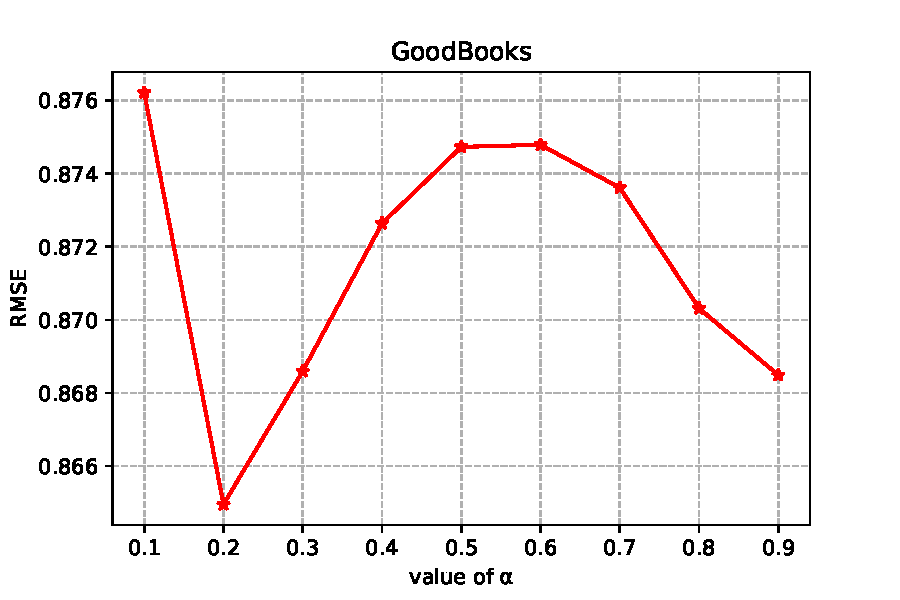
\includegraphics[width=0.2\textwidth]{imgs/alpha_1.pdf}
	}
	\quad
	\subfigure{
		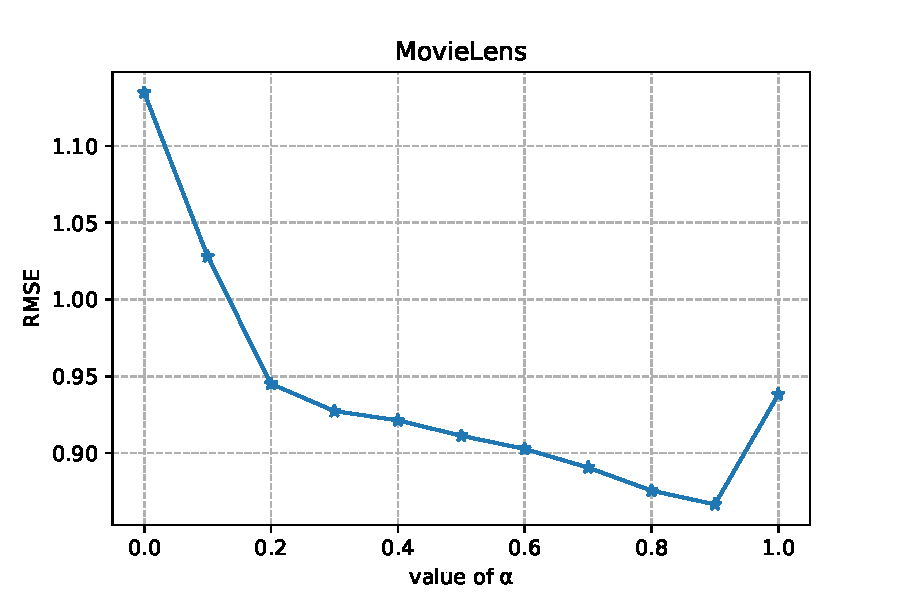
\includegraphics[width=0.2\textwidth]{imgs/alpha_2.pdf}
	}
	\quad
	\subfigure{
		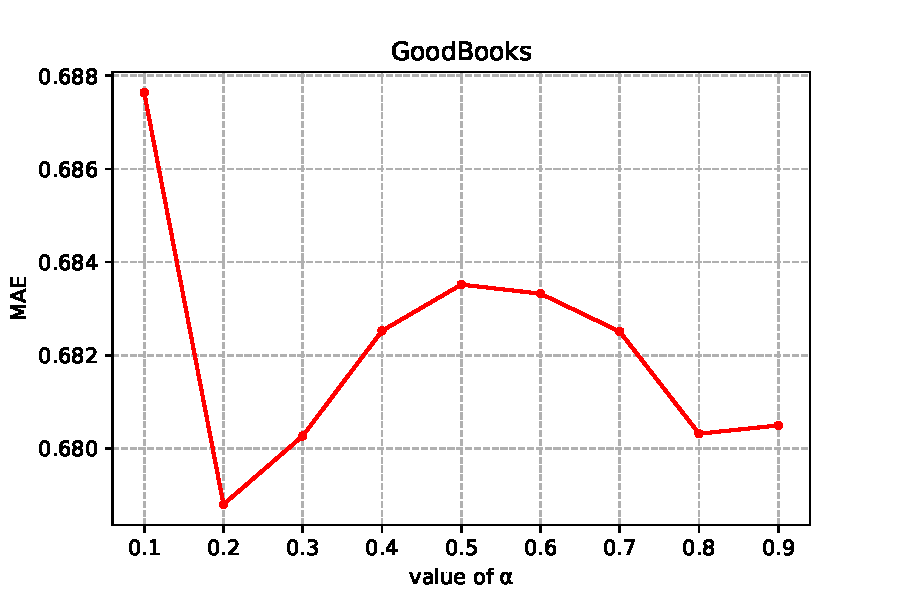
\includegraphics[width=0.2\textwidth]{imgs/alpha_3.pdf}
	}
	\quad
	\subfigure{
		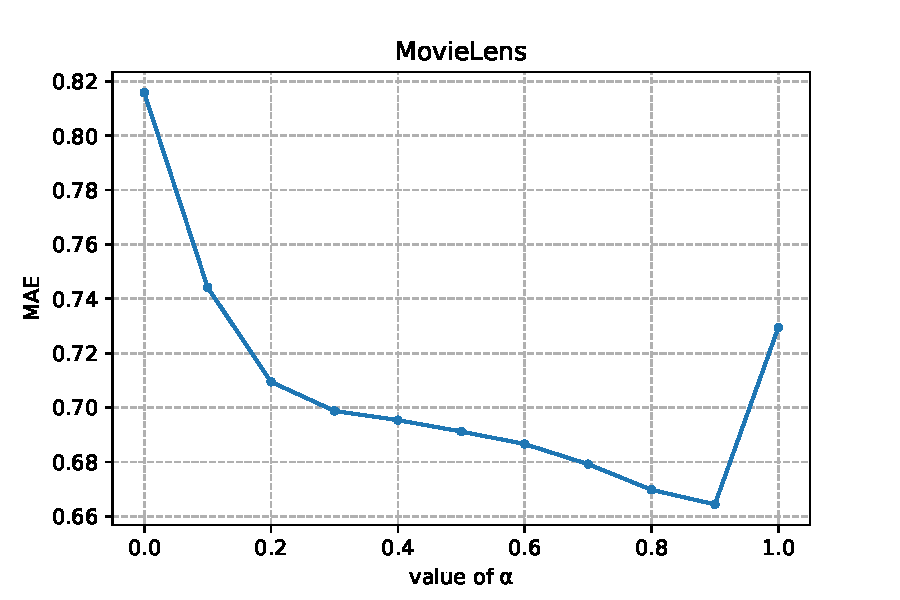
\includegraphics[width=0.2\textwidth]{imgs/alpha_4.pdf}
	}
	\caption{ the inspect of Value $ \alpha $\label{fig:alpha}} 
\end{figure}

\textbf{阈值的影响}。 研究阈值对模型的影响。结果如图\ref{fig:threshold}
\begin{figure}[htbp]
	\centering
	\subfigure{
		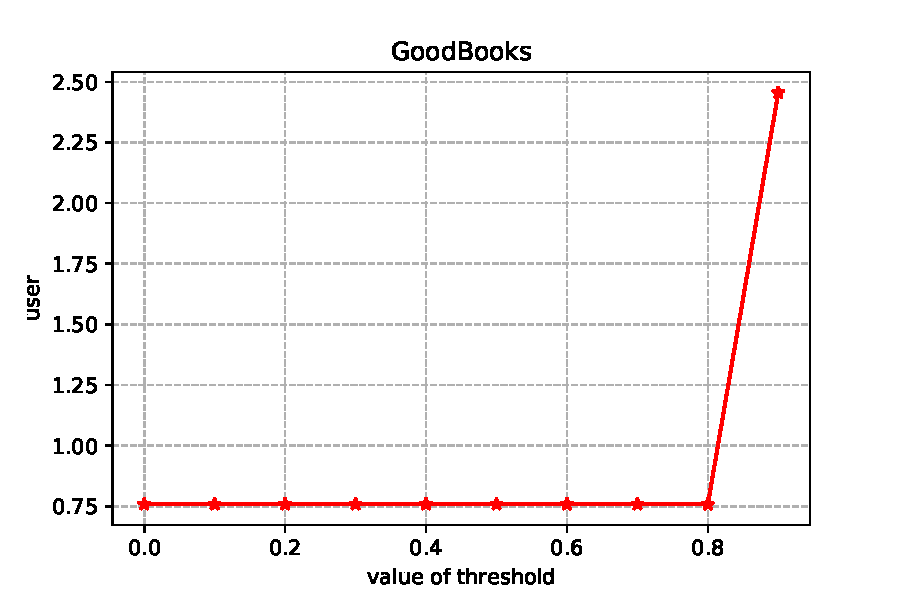
\includegraphics[width=0.2\textwidth]{imgs/threshold_1.pdf}
	}
	\quad
	\subfigure{
		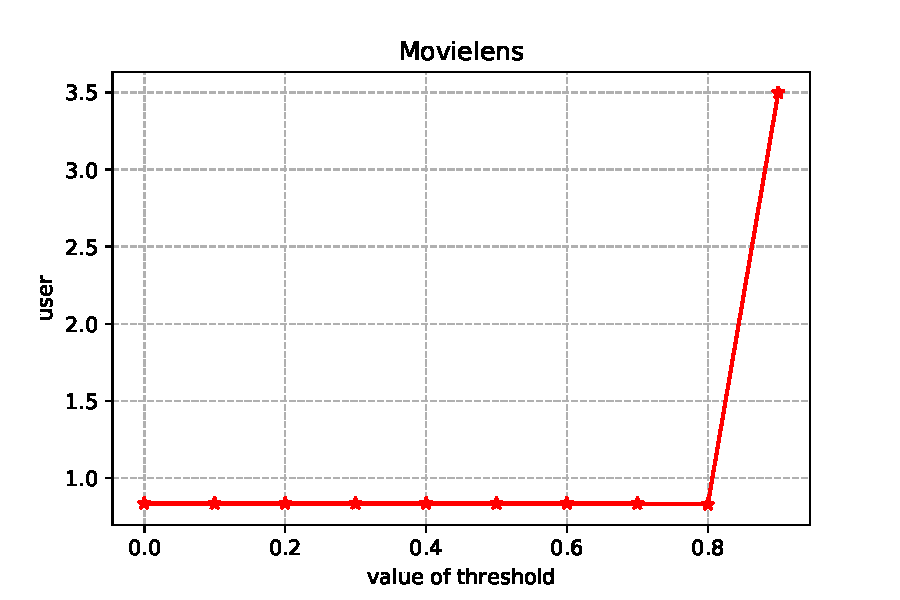
\includegraphics[width=0.2\textwidth]{imgs/threshold_2.pdf}
	}
	\quad
	\subfigure{
		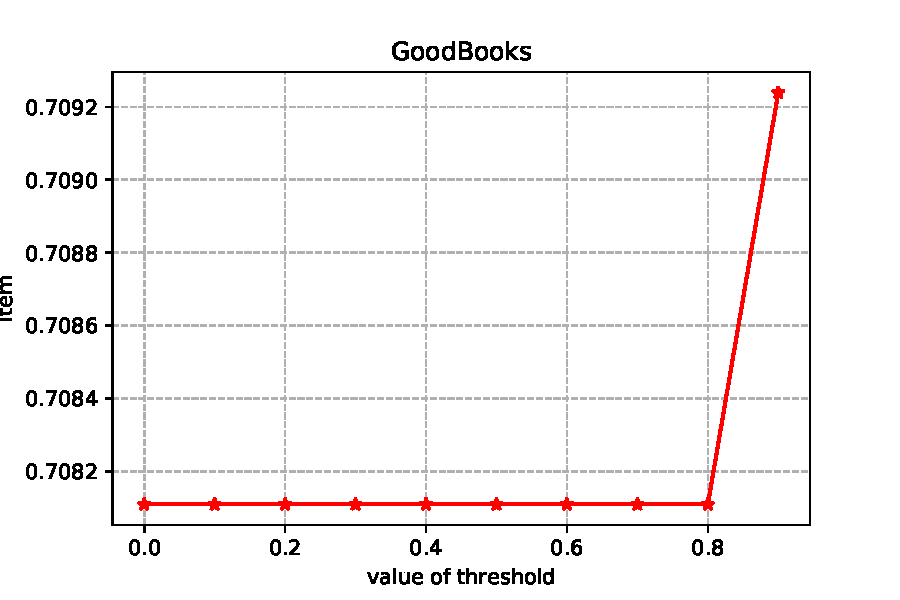
\includegraphics[width=0.2\textwidth]{imgs/threshold_3.pdf}
	}
	\quad
	\subfigure{
		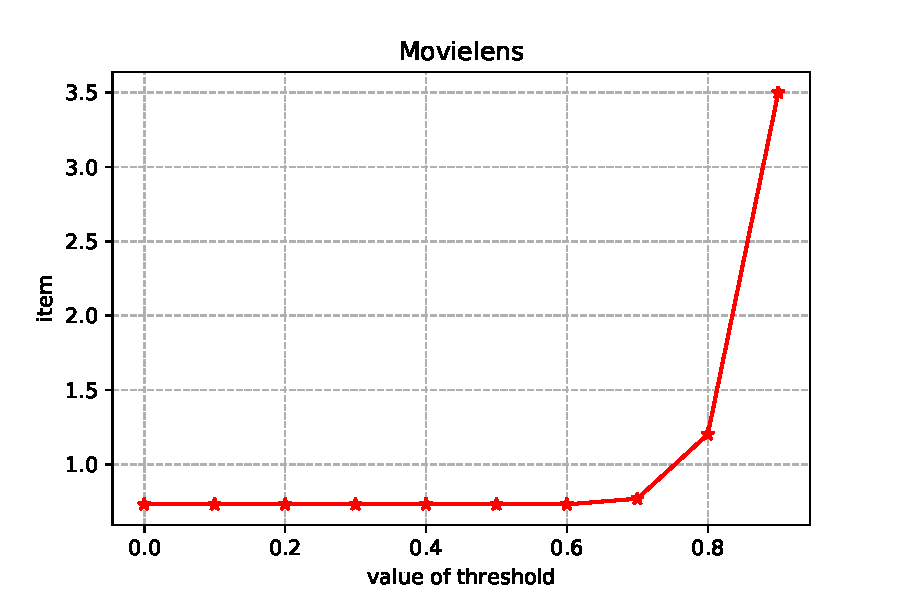
\includegraphics[width=0.2\textwidth]{imgs/threshold_4.pdf}
	}
	\caption{ the inspect of Value Density \label{fig:threshold}} 
\end{figure}


\textbf{联合训练时矩阵维度的影响}。 联合训练时矩阵维度对模型的影响。结果如图\ref{fig:Density}
\begin{figure}[htbp]
	\centering
	\subfigure{
		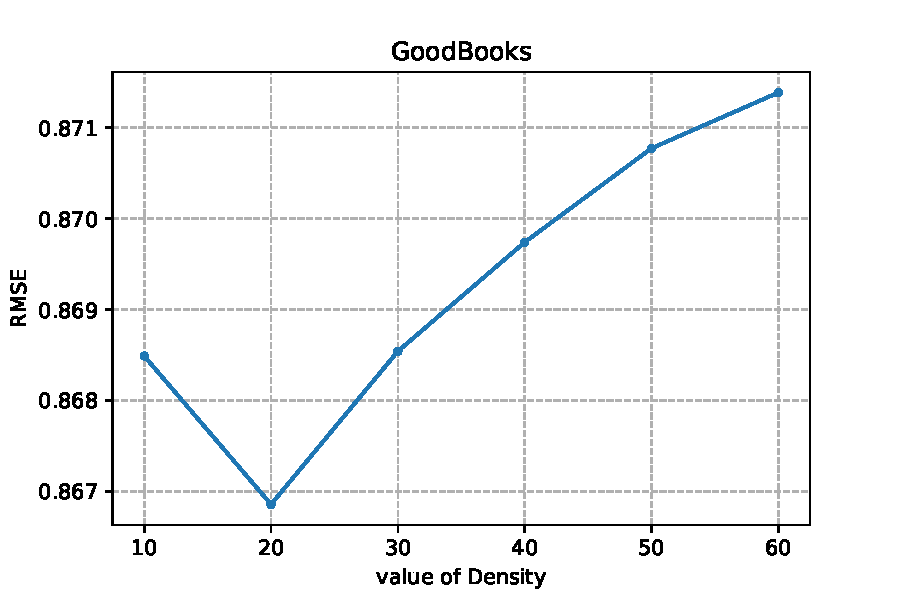
\includegraphics[width=0.2\textwidth]{imgs/Density_1.pdf}
	}
	\quad
	\subfigure{
		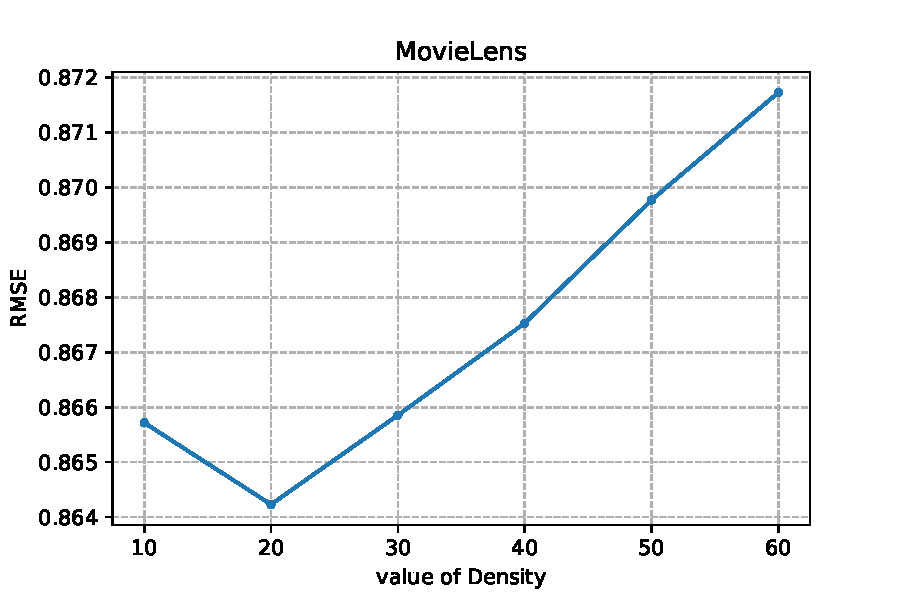
\includegraphics[width=0.2\textwidth]{imgs/Density_2.pdf}
	}
	\quad
	\subfigure{
		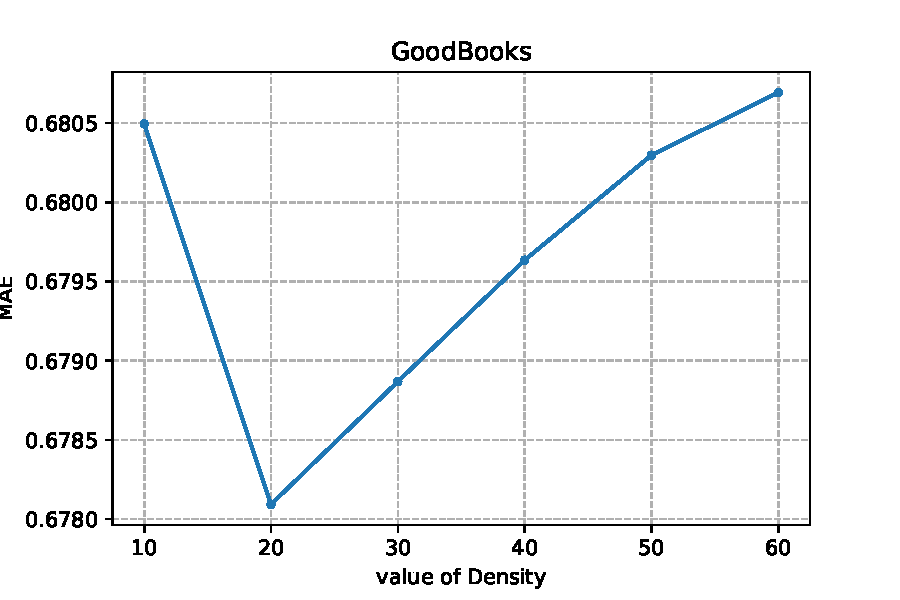
\includegraphics[width=0.2\textwidth]{imgs/Density_3.pdf}
	}
	\quad
	\subfigure{
		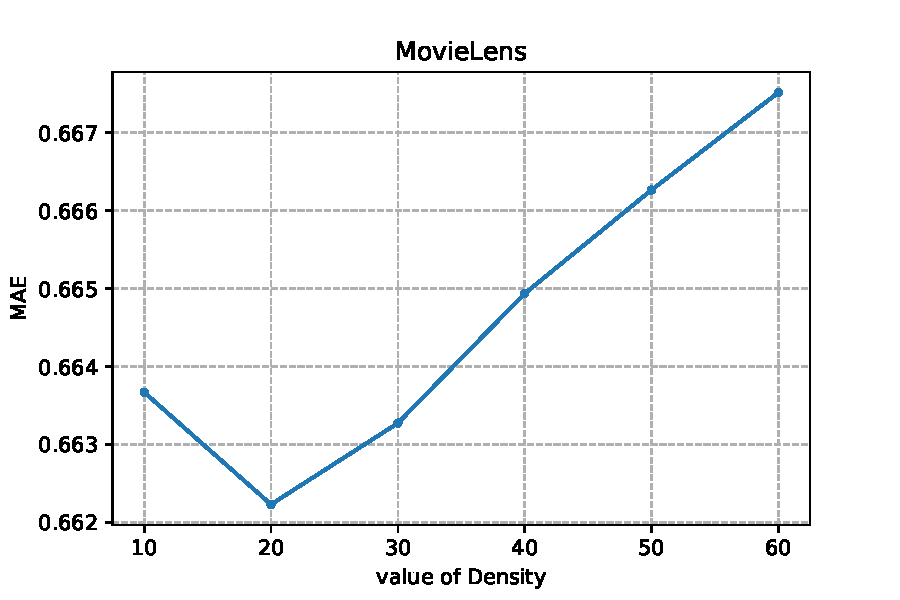
\includegraphics[width=0.2\textwidth]{imgs/Density_4.pdf}
	}
	\caption{ the inspect of Value Density \label{fig:Density}} 
\end{figure}


\section{结论}
结论部分,介绍论文的实验结果

\bibliographystyle{unsrt}
\bibliography{wpref}

\end{document}
